\documentclass[9pt,xcolor=table]{beamer}
\usetheme{Warsaw}

\usepackage{xcolor}
\usepackage{xltxtra}
\usepackage{dirtree}
\usepackage{ragged2e}
\usepackage{listings}
\usepackage{graphicx}
\usepackage{chronology}

\lstset{
    language=Bash, % Define a linguagem do código como Bash
    backgroundcolor=\color{black!5}, % Cor de fundo
    basicstyle=\footnotesize\ttfamily\color{black}, % Estilo básico do texto
    keywordstyle=\color{blue}, % Estilo das palavras-chave
    stringstyle=\color{red}, % Estilo das strings
    commentstyle=\color{green!70!black}, % Estilo dos comentários
    numbers=none, % Posição dos números de linha
    numberstyle=\tiny\color{gray}, % Estilo dos números de linha
    stepnumber=1, % Incremento dos números de linha
    numbersep=5pt, % Espaçamento dos números de linha
    showspaces=false, % Mostrar espaços com um sublinhado
    showstringspaces=false, % Mostrar espaços em strings com um sublinhado
    showtabs=false, % Mostrar tabulações com um sublinhado
    frame=single, % Moldura em volta do código
    rulecolor=\color{black}, % Cor da moldura
    tabsize=2, % Tamanho da tabulação
    captionpos=b, % Posição da legenda abaixo do código
    breaklines=true, % Quebra automática de linha
    breakatwhitespace=false, % Quebra somente em espaços em branco
    escapeinside={\%*}{*)}, % Permite adicionar LaTeX dentro do código
    morekeywords={*,...} % Adicionar mais palavras-chave
}

\date{20 de maio de 2023}
\title{OpenBSD: Segurança e Inovação em SOs}
\institute[PUC]{Pontifícia Universidade Católica de Minas Gerais}
\logo{
\includegraphics[width=0.7cm]{imagens/logo_pucminas.png}}
\author[Gustavo, Hernane, João Víctor, Pedro]{Gustavo Valadares \and Hernane Rosa \and João Martins \and Pedro Igor}

\begin{document}

\begin{frame}
  \titlepage
\end{frame}
\begin{frame}{Introdução}
  \begin{itemize}
    \item O que é o OpenBSD?
    \item Breve histórico do projeto
    \item Objetivos do OpenBSD
  \end{itemize}
\end{frame}
\begin{frame}{O que é o OpenBSD?}
  \begin{itemize}
    \item OpenBSD é um sistema operacional livre e de código aberto baseado no ramo BSD. \pause
    \item Destaca-se por sua ênfase em segurança, portabilidade e código limpo. \pause
    \item Desenvolvido desde 1995 por uma comunidade global liderada por Theo de Raadt. \pause
    \item Utiliza uma licença permissiva (licença BSD), permitindo modificações e distribuição livre. \pause
    \item Amplamente adotado em servidores, roteadores, estações de trabalho e dispositivos embarcados.
  \end{itemize}
\end{frame}
\begin{frame}{O que é o OpenBSD?}
    \begin{columns}
        \begin{column}{0.3\textwidth}
            \centering
            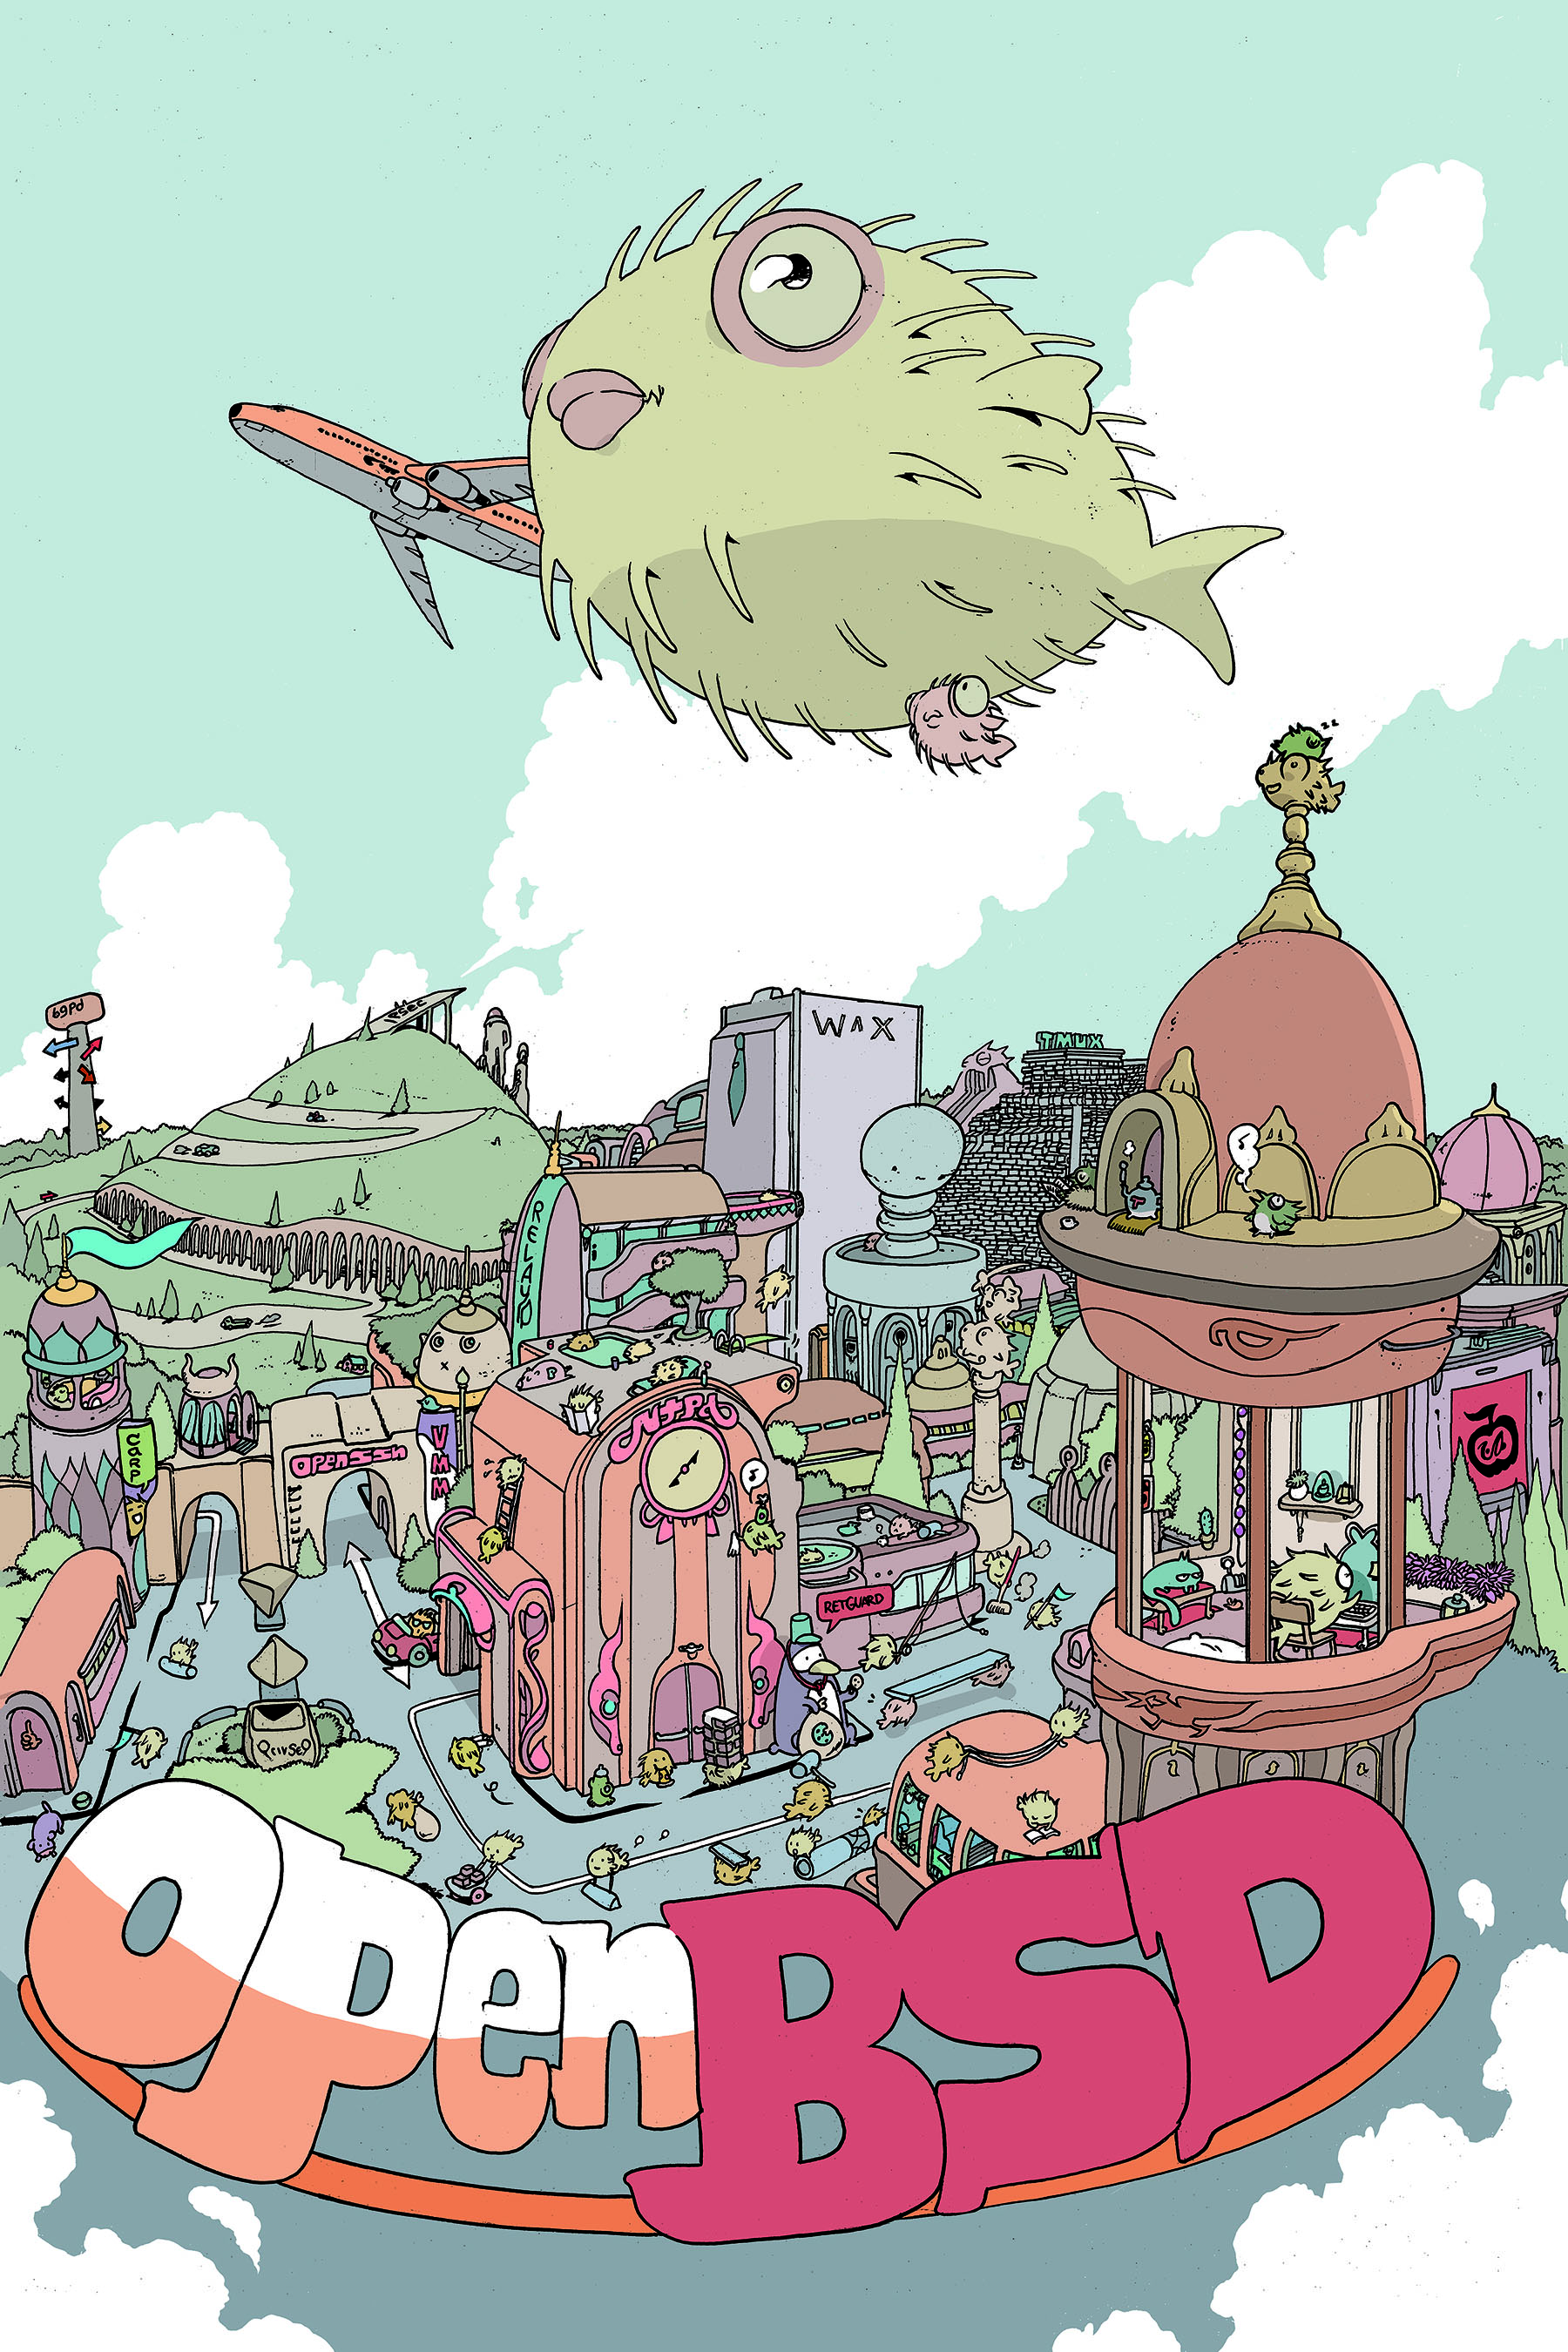
\includegraphics[width=\textwidth]{imagens/openbsd-fan.jpg}
        \end{column}
        \begin{column}{0.3\textwidth}
            \centering
            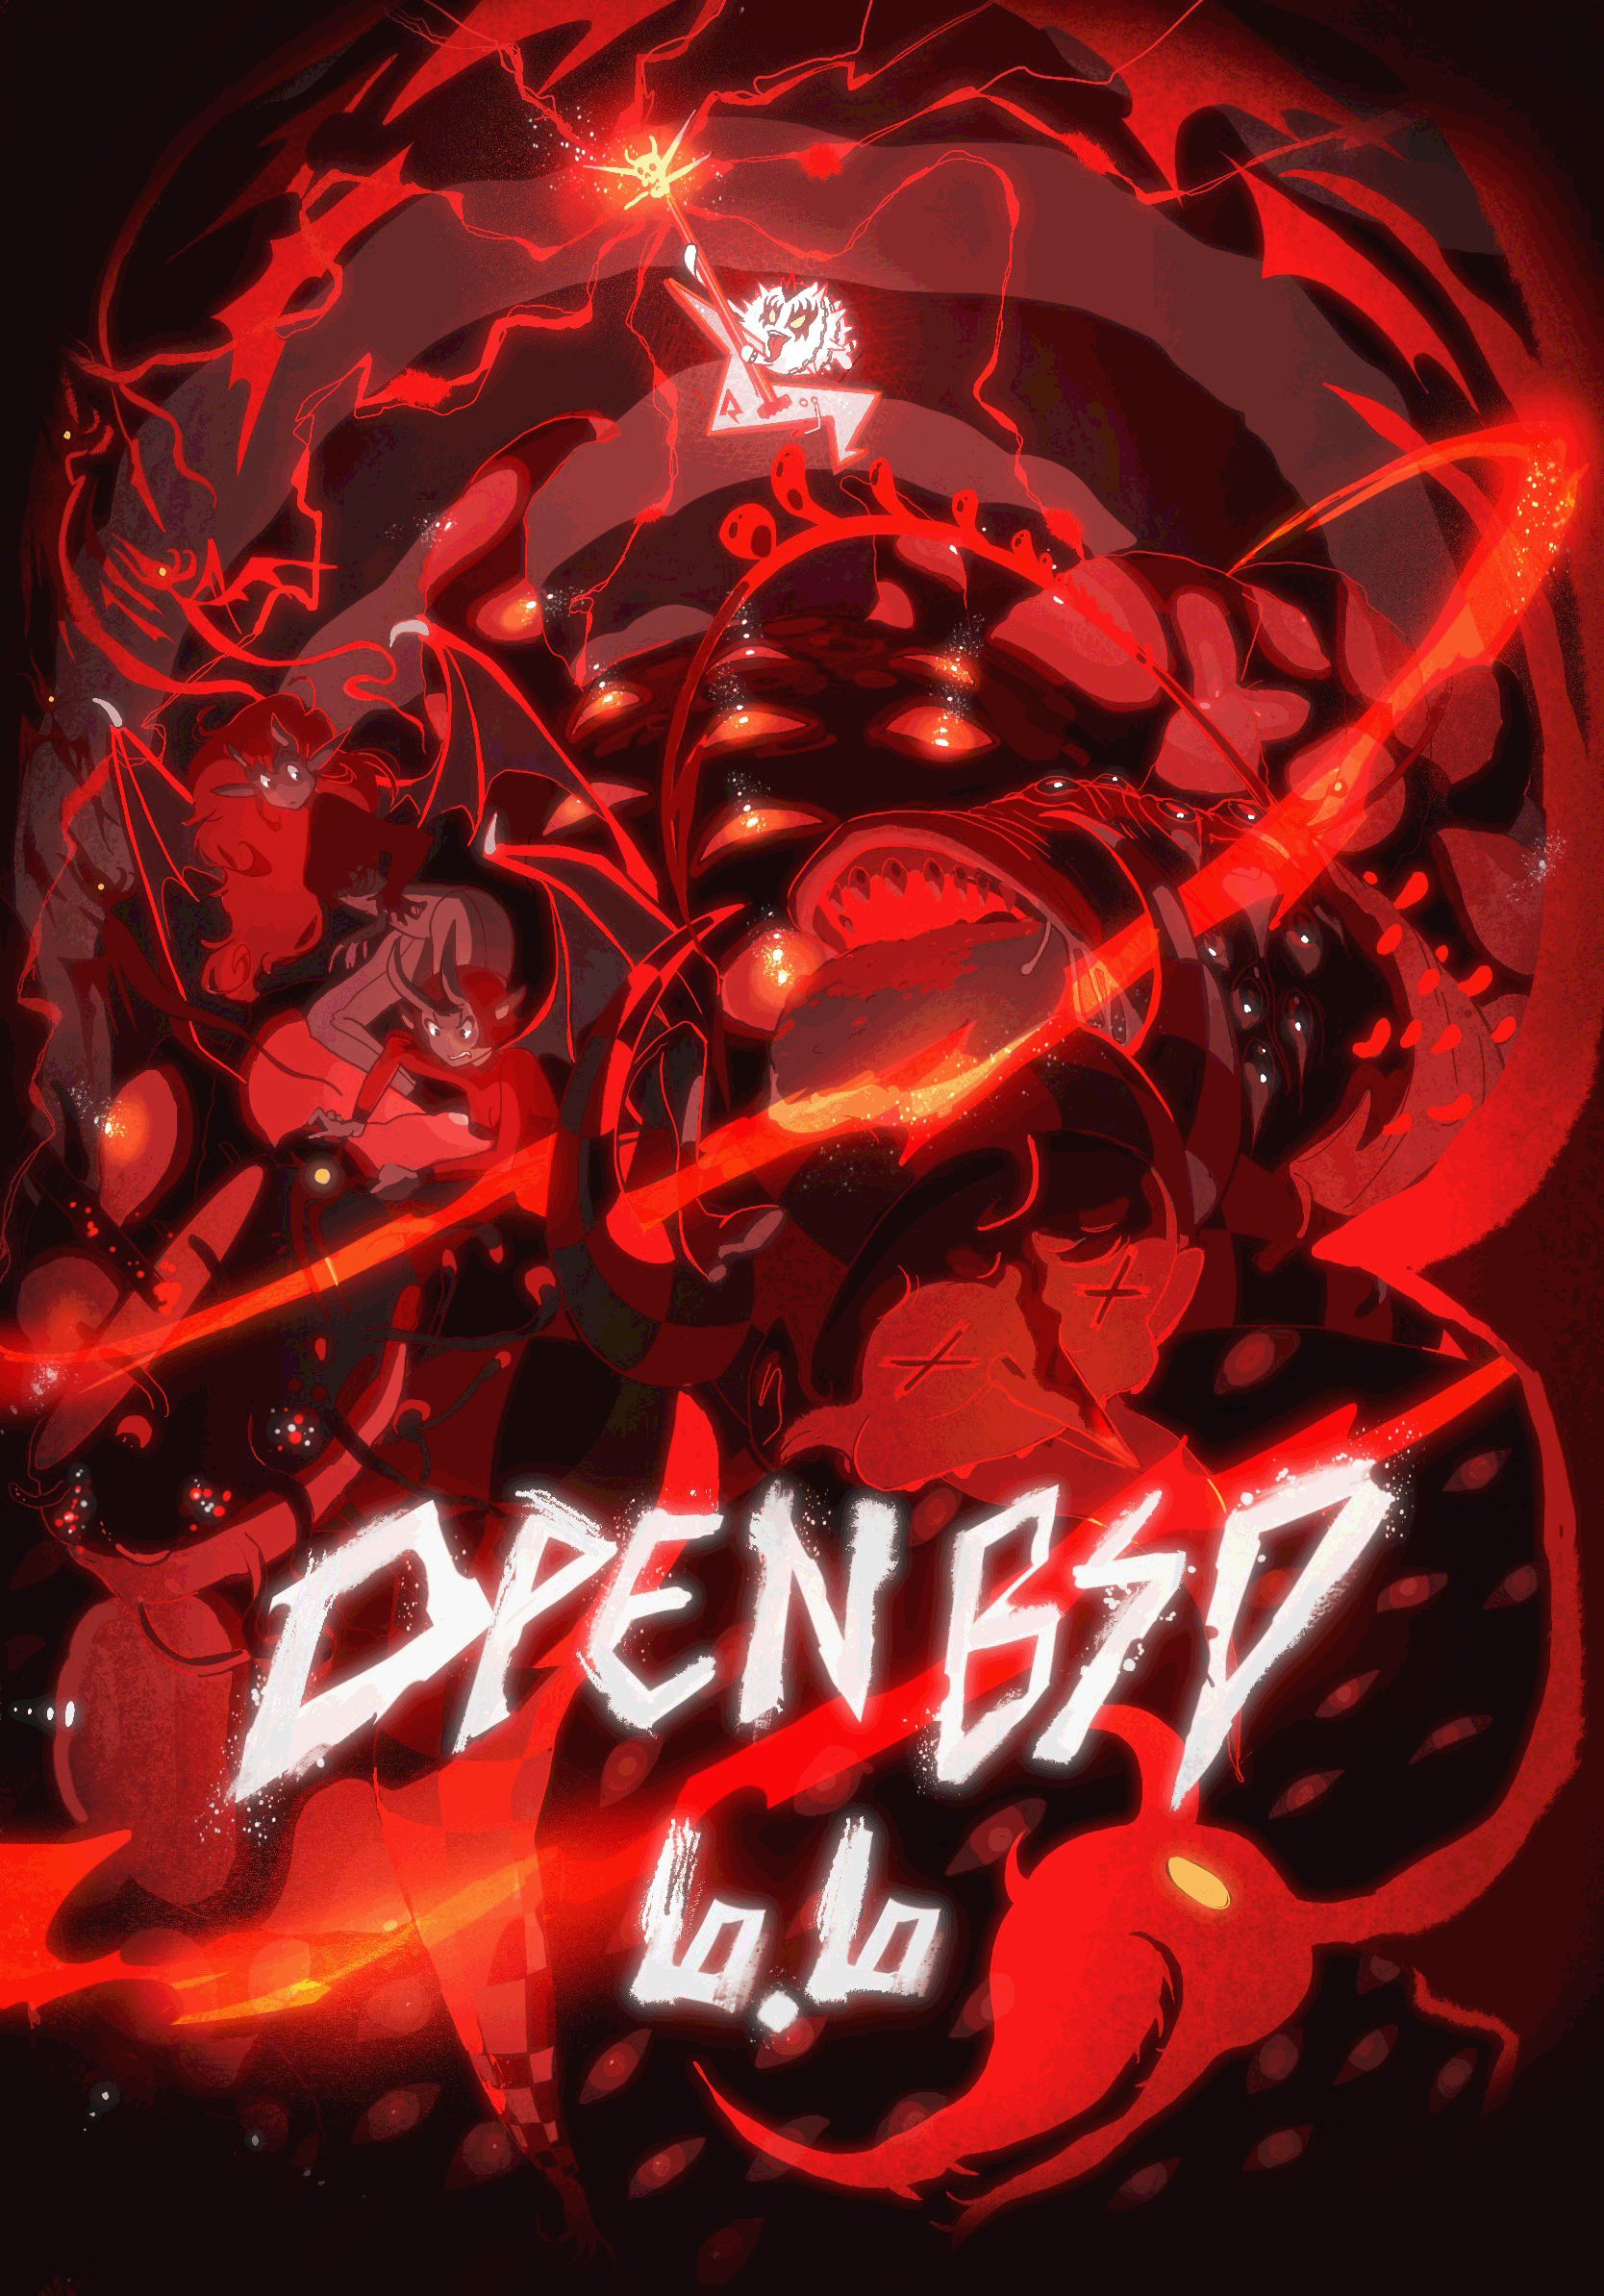
\includegraphics[width=\textwidth]{imagens/banner-openbsd.png}
        \end{column}
        \begin{column}{0.3\textwidth}
            \centering
            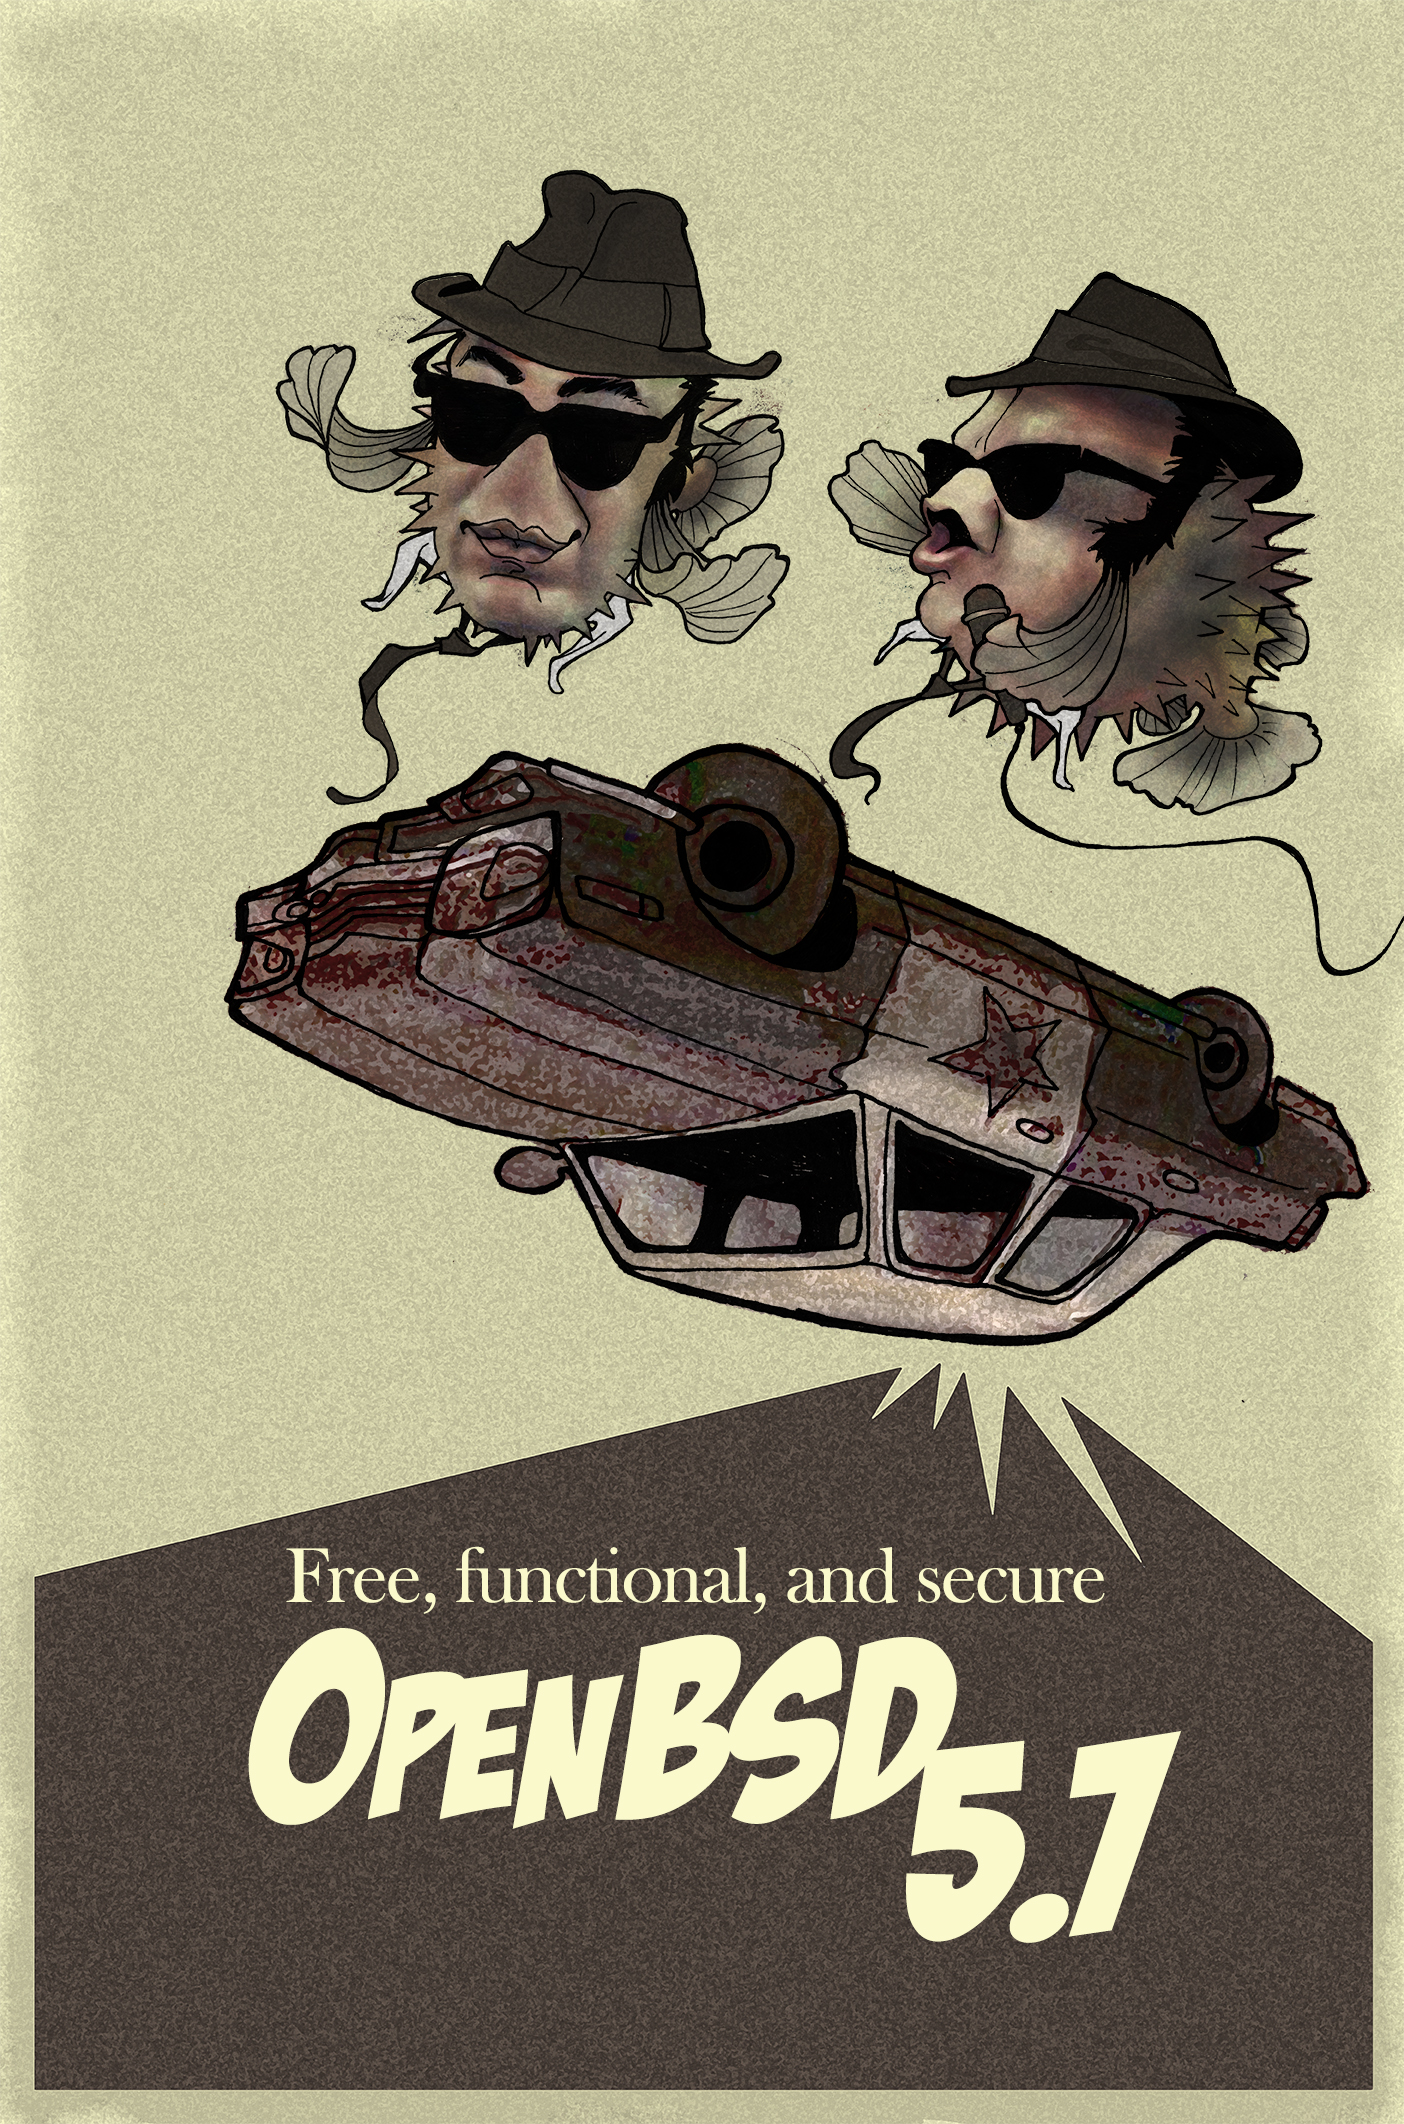
\includegraphics[width=\textwidth]{imagens/openbsd-poster.jpg}
        \end{column}
    \end{columns}
\end{frame}
\begin{frame}{História do OpenBSD}
\begin{chronology}[5]{1995}{2022}{\textwidth}
\event[1995]{1995}{Início do desenvolvimento}\pause
\event[1997]{1997}{OpenBSD Ports}\pause
\event[1999]{1999}{OpenSSH}\pause
\event[2002]{2002}{OpenNTPD}\pause
\event[2005]{2005}{Sshguard}\pause
\event[2012]{2012}{OpenBSD Foundation}\pause
\event[2015]{2015}{LibreSSL}\pause
\event[2020]{2020}{OpenRSYNC}
\end{chronology}
\end{frame}
\begin{frame}[fragile]
\frametitle{Introdução ao OpenBSD Ports}
\justifying
O sistema de Ports do OpenBSD é uma ferramenta poderosa que simplifica a instalação de software de terceiros. Ele permite que os usuários instalem e atualizem aplicativos de maneira fácil e eficiente.
\vspace{0.5cm}
\begin{lstlisting}
$ cd /tmp
$ ftp https://cdn.openbsd.org/pub/OpenBSD/$(uname -r)/{ports.tar.gz,SHA256.sig}
$ signify -Cp /etc/signify/openbsd-$(uname -r | cut -c 1,3)-base.pub -x SHA256.sig ports.tar.gz
\end{lstlisting}
\end{frame}
\begin{frame}[fragile]
\frametitle{Estrutura e Uso dos Ports}
\justifying
Cada \textbf{port} é essencialmente um conjunto de metadados que descreve como baixar, descompactar, corrigir, compilar e instalar um aplicativo. O diretório de ports (\verb|/usr/ports|) contém uma subpasta para cada aplicativo disponível.
\vspace{0.5cm}
\dirtree{%
.1 /usr/ports.
.2 net.
.3 rsnapshot.
.4 Makefile.
.4 distinfo.
.4 patches.
.4 files.
.4 pkg.
.4 README.
.3 \ldots.
}
\end{frame}
\begin{frame}[fragile]
\frametitle{Estrutura e Uso dos Ports (Continuação)}
\justifying
Para instalar um aplicativo usando ports, você navega até a subpasta correspondente e executa \verb|make install|. Isso baixará o código-fonte do aplicativo, aplicará quaisquer patches necessários, compilará o código-fonte e instalará o aplicativo.
\vspace{0.5cm}
\begin{lstlisting}
$ make install
===>  Checking files for rsnapshot-1.4.2
>> Fetch https://github.com/rsnapshot/rsnapshot/archive/1.4.2/rsnapshot-1.4.2.tar.gz
100% |**************************************************|   365 KB    00:02
>> (SHA256) rsnapshot-1.4.2.tar.gz: OK
===> rsnapshot-1.4.2 depends on: metaauto-* - not found
[...]
===>  Installing rsnapshot-1.4.2 from /build/source/ports/packages/amd64/all/
rsnapshot-1.4.2: ok
\end{lstlisting}
\end{frame}
\begin{frame}
\frametitle{Importância dos Ports}
\justifying
Os Ports são uma parte essencial do ecossistema OpenBSD. Eles permitem que os usuários se beneficiem de uma ampla gama de software de terceiros, sem a necessidade de rastrear e compilar o código-fonte manualmente. Além disso, como o sistema de Ports cuida de todas as dependências, ele garante que cada aplicativo funcione corretamente após a instalação.
\vspace{0.5cm}
\begin{columns}
\begin{column}{0.3\textwidth}
\centering

\includegraphics[width=0.5\textwidth]{imagens/hydra-logo.png}
\end{column}
\begin{column}{0.3\textwidth}
\centering

\includegraphics[width=0.5\textwidth]{imagens/mpv-logo.png}
\end{column}
\begin{column}{0.3\textwidth}
\centering

\includegraphics[width=0.5\textwidth]{imagens/kde-logo.png}
\end{column}
\end{columns}
\end{frame}
\begin{frame}[fragile]
\frametitle{Introdução ao OpenSSH}
\textbf{OpenSSH} (\textit{Open Secure Shell}) é um conjunto de ferramentas de conectividade de computador que fornecem criptografia de comunicações em uma rede de computadores. Ele foi criado como um projeto do OpenBSD e é padrão em muitos sistemas operacionais Unix-like.
\vspace{0.5cm}
\begin{lstlisting}
pigor@gigabyte > $ ssh root@192.168.1.9
root@192.168.1.9's password:
[....]
root@192.168.1.9 > #
\end{lstlisting}
\end{frame}
\begin{frame}[fragile]
\frametitle{OpenNTPD}
\justifying
\textbf{OpenNTPD} é uma implementação simples e segura do Protocolo de Tempo de Rede (\textit{Network Time Protocol - NTP}). Foi desenvolvido como parte do projeto OpenBSD com o objetivo de ser tão seguro, fácil de usar e livre de bugs quanto possível.
\vspace{0.5cm}
\begin{lstlisting}
$ grep ntpd /var/log/daemon.log | grep adjusting
May 10 03:32:20 pigor ntpd[4784]: adjusting local clock by -1.162333s
May 10 03:36:08 pigor ntpd[4784]: adjusting local clock by -1.023899s
May 10 03:40:02 pigor ntpd[4784]: adjusting local clock by -0.902637s
May 10 03:43:43 pigor ntpd[4784]: adjusting local clock by -0.789431s
May 10 03:47:35 pigor ntpd[4784]: adjusting local clock by -0.679320s
May 10 03:50:45 pigor ntpd[4784]: adjusting local clock by -0.605858s
May 10 03:53:31 pigor ntpd[4784]: adjusting local clock by -0.529821s
\end{lstlisting}
\end{frame}
\begin{frame}{Princípios do OpenBSD}
  \begin{itemize}
    \item Segurança como prioridade
    \item Código limpo e revisões extensivas
    \item Acesso aberto e colaborativo
    \item Documentação abrangente
  \end{itemize}
\end{frame}
\begin{frame}{Recursos de Segurança}
  \begin{itemize}
    \item Modelo de desenvolvimento e revisões de código;
    \item Análise de segurança proativa;
    \item Mecanismos de mitigação de ataques;
    \item Uso do OpenSSH como padrão;
    \item Política padrão "secure by default".
  \end{itemize}
\end{frame}
\begin{frame}
\frametitle{Introdução à "Segurança por padrão"}
\justifying
A política de \textbf{Segurança por padrão} do OpenBSD significa que, na instalação padrão, todos os serviços não essenciais serão desativados. O sistema operacional é configurado para ser seguro "fora da caixa", reduzindo a área de ataque e protegendo os usuários contra ameaças de segurança.
\vspace{0.5cm}
\begin{enumerate}
 \item W\^{}X;
 \item Address Space Layout Randomization;
 \item ProPolice (uma proteção de estouro de buffer).
\end{enumerate}
\end{frame}
\begin{frame}[fragile]
\frametitle{ASLR}
\justifying
\textbf{Address Space Layout Randomization} (\textit{ASLR}) é uma técnica de segurança que evita alguns tipos de ataques, como ataques de execução de código e estouro de buffer. Ele faz isso ao randomizar o layout do espaço de endereços de um processo, tornando mais difícil para um atacante prever o local de um determinado pedaço de código.
\vspace{0.5cm}
\begin{lstlisting}[language=C]
int global_variable = 42;

int main() {
    int local_variable = 123;
    printf("Endereço da variável global: %p\n", &global_variable);
    printf("Endereço da variável local: %p\n", &local_variable);
    return 0;
}
\end{lstlisting}
\end{frame}
\begin{frame}[fragile]
\frametitle{ASLR}
\justifying
A variável global chamada \verb|global_variable| e uma variável local chamada \verb|local_variable|. O programa imprime os endereços de memória dessas variáveis usando o especificador de formato \verb|%p| da função \verb|printf()|.

\begin{lstlisting}
$ gcc -o aslr_example aslr_example.c
$ ./aslr_example                              # 1ª Tentativa
Endereço da variável global: 0x7f7ce5a19034
Endereço da variável local: 0x7ffeb330ca1c
\end{lstlisting}
\vspace{0.1cm}
Ao compilar e executar esse código no OpenBSD, você verá que os endereços de memória das variáveis serão diferentes a cada execução. Isso ocorre porque o ASLR está em ação, randomizando a localização das variáveis na memória.
\begin{lstlisting}
$ ./aslr_example                              # 2ª Tentativa
Endereço da variável global: 0x7f4ed2923034
Endereço da variável local: 0x7ffedc9db81c
\end{lstlisting}
\end{frame}
\begin{frame}[fragile]
\frametitle{W\^{}X}
\justifying
OpenBSD implementa a política \textbf{W\^{}X} por padrão. Isso significa que, por padrão, todas as páginas de memória no sistema são configuradas para serem ou graváveis ou executáveis, mas nunca ambas. Esta política é implementada em todos os níveis do sistema, desde o kernel até os aplicativos de espaço do usuário.
\vspace{0.5cm }
\begin{lstlisting}[language=C]
void function() {
    printf("Esta é uma função protegida pelo W^X.\n");
    char* writable_memory = (char*)function;
    writable_memory[0] = 'X';
}

int main() {
    void (*function_ptr)() = &function;
    function_ptr();
    return 0;
}
\end{lstlisting}

\end{frame}
\begin{frame}[fragile]
\frametitle{ProPolice}
\justifying
\textbf{ProPolice} é uma extensão do compilador GCC que ajuda a prevenir estouros de buffer, um tipo comum de vulnerabilidade de segurança. Faz isso rearranjando a pilha de memória para tornar mais difícil para um atacante sobrescrever os dados importantes.
\vspace{0.5cm}
\begin{lstlisting}[language=C]
void vulnerable_function(char* input) {
    char buffer[10];
    strcpy(buffer, input);
    printf("Buffer: %s\n", buffer);
}

int main() {
    char input[20];
    printf("Digite um texto: ");
    fgets(input, sizeof(input), stdin);
    vulnerable_function(input);
    return 0;
}
\end{lstlisting}
\end{frame}
\begin{frame}[fragile]
\frametitle{ProPolice}
\justifying
A função chamada \verb|vulnerable_function| que copia o conteúdo da entrada do usuário para um buffer local sem verificar o tamanho do input. Isso pode levar a um estouro de pilha se o usuário fornecer uma entrada maior do que o tamanho do buffer.
\begin{lstlisting}
user@openbased > $ gcc -fstack-protector -o propolice_example
\end{lstlisting}
O OpenBSD compila o código com a opção de compilador \verb|-fstack-protector|, que adiciona um mecanismo de proteção ao estouro de pilha. Quando ativado, esse mecanismo verifica se o estouro de pilha ocorreu antes de permitir que a função retorne. Se o estouro de pilha for detectado, o programa será encerrado imediatamente.
\begin{lstlisting}
user@openbased > $ ./propolice_example
Digite um texto: Hello, Propolice!
Buffer: Hello, Prop
\end{lstlisting}
\end{frame}
\begin{frame}[fragile]
\frametitle{ProPolice}
Como dito, a \verb|string| continha apenas 10 caracteres e, por proteção, o programa será encerrado após violar o limite determinado.
\vspace{0.5cm}
\begin{table}[]
\begin{tabular}{|cccccccccc
>{\columncolor[HTML]{FFFC9E}}c
>{\columncolor[HTML]{FFFC9E}}c
>{\columncolor[HTML]{FFFC9E}}c
>{\columncolor[HTML]{FFFC9E}}c
>{\columncolor[HTML]{FFFC9E}}c
>{\columncolor[HTML]{FFFC9E}}c|}
\hline
H & e & l & l & o & , & P & r & o & p & \textbf{o}                & \textbf{l}                & \textbf{i}                & \textbf{c}                & \textbf{e}                & \textbf{!}                \\ \hline
0 & 1 & 2 & 3 & 4 & 5 & 6 & 7 & 8 & 9 & {\color[HTML]{FE0000} 10} & {\color[HTML]{FE0000} 11} & {\color[HTML]{FE0000} 12} & {\color[HTML]{FE0000} 13} & {\color[HTML]{FE0000} 14} & {\color[HTML]{FE0000} 15} \\ \hline
\end{tabular}
\end{table}
\end{frame}
\begin{frame}{Recursos de Inovação}
  \begin{itemize}
    \item Virtualização com o VMM;
    \item Ferramentas e utilitários exclusivos;
    \item Foco na simplicidade e no desempenho;
    \item Suporte a sistemas de arquivos criptografados.
    \item Portabilidade e suporte a diversas arquiteturas;
  \end{itemize}
\end{frame}
\begin{frame}{Comunidade e Contribuições}
  \begin{itemize}
    \item Doações e financiamento.
    \item Auditoria de código externa;
    \item \textit{Mailing lists} e conferências anuais;
    \item Colaboração com outros projetos de código aberto;
  \end{itemize}
\end{frame}
\begin{frame}{Conclusão}
  \begin{itemize}
    \item OpenBSD: Segurança e Inovação;
    \item Comprometimento com a qualidade e a confiabilidade;
    \item Sistema operacional confiável para diversos casos de uso.
  \end{itemize}
\end{frame}
\begin{frame}
  \frametitle{Bibliografia}

  \begin{itemize}
    \item Hartmeier, Daniel, and Systor, AG. "Design and Performance of the OpenBSD Stateful Packet Filter (pf)." In USENIX Annual Technical Conference, FREENIX Track, pp. 171--180, 2002.
    \item Marco-Gisbert, Hector, and Ripoll Ripoll, Ismael. "Address space layout randomization next generation." In Applied Sciences, vol. 9, no. 14, p. 2928, 2019.
    \item Izurieta, Clemente, and Bieman, James. "The evolution of FreeBSD and Linux." In Proceedings of the 2006 ACM/IEEE international symposium on empirical software engineering, pp. 204--211, 2006.
    \item Hsu, Jeffrey M. "The dragonflybsd operating system." In Proceedings USENIX AsiaBSDCon, Taipei, Taiwan, 2004.
    \item Mewburn, Luke. "The Design and Implementation of the NetBSD rc. d System." In USENIX Annual Technical Conference, FREENIX Track, pp. 69--79, 2001.
  \end{itemize}
\end{frame}
\end{document}
